% Numbers come from artifacts/reported_results/2026-10-04-rollout-fidelity/ (see its README).
% Generated by artifacts/reported_results/2026-10-04-rollout-fidelity/generate.py; do not edit.
\newcommand{\RFMainGenerate}{49.2}
\newcommand{\RFFixGenerate}{36.8}
\newcommand{\RFPackGenerate}{28.4}
\newcommand{\RFFixSaving}{25\%}
\newcommand{\RFPackSaving}{22\%}
\newcommand{\RFTotalSaving}{42\%}
\newcommand{\RFMainReward}{2.80}
\newcommand{\RFFixReward}{4.62}
\newcommand{\RFPostFixRewardMin}{4.45}
\newcommand{\RFPostFixRewardMax}{4.77}
\newcommand{\RFLongTailRollout}{2}
\newcommand{\RFWorkerKv}{5938}
\newcommand{\RFTrainerKv}{2263}
\newcommand{\RFRatioBuggy}{5.0}
\newcommand{\RFRatioHealthy}{3.4}
\newcommand{\RFTailMin}{1.16}
\newcommand{\RFTailMax}{1.84}
\newcommand{\RFSmallBase}{99.3}
\newcommand{\RFSmallOverlap}{93.7}
\newcommand{\RFSmallSteal}{77.4}
\newcommand{\RFSmallBoth}{71.5}
\newcommand{\RFSmallBothSaving}{28\%}
\newcommand{\RFLargeBase}{128.4}
\newcommand{\RFLargeSteal}{131.1}
\newcommand{\RFLargeFirstBase}{118.3}
\newcommand{\RFLargeFirstSteal}{131.5}
\newcommand{\RFLargeTail}{90.8}
\newcommand{\RFLargeTailSteal}{68.4}
\newcommand{\RFTtoiBase}{150.2}
\newcommand{\RFTtoiBalanced}{108.6}
\newcommand{\RFTtoiIdle}{29\%}
\newcommand{\RFNaiveBalanced}{133.9}
\newcommand{\RFNaiveSteal}{115.9}
\newcommand{\RFNaiveGap}{25}
\newcommand{\RFStealRecovered}{18}
\newcommand{\RFPackedGroupEight}{13.96}
\newcommand{\RFUnpackedGroupEight}{18.04}


\section{Rollout Fidelity and Request Shaping}
\label{sec:fidelity}

Section~\ref{sec:reward} took the generated sample as given and asked where its reward should be computed.
This section looks at the sample itself.
Two properties of a rollout decide whether the reward and the gradient refer to the same thing, and what the rollout costs: the engine and the trainer must condition on the same sequence, and the engine's request must be shaped so that one request is not one sample when a group of siblings would do.
Both are visible only through the engine's own boundary, which is where a lineage-preserving trajectory does not help: the \sample{} that comes back is well formed either way.

\paragraph{Source scope.}
Four changes to the vLLM-Omni BAGEL path, proposed as UniRL pull requests~\#547--\#550 and open at the time of writing.
They are stacked in that order and must land in it.
Every measurement below is ours, on one eight-GPU H20 node, and the per-run records and generator are under \codepath{artifacts/reported\_results/2026-10-04-rollout-fidelity/}.
The scheduling experiment of Section~\ref{sec:fidelity-tail} is on a branch with no pull request.

\subsection{A conditioning mismatch that the importance ratio could not see}
\label{sec:fidelity-layout}

In image editing the policy conditions on a source image.
UniRL builds that conditioning itself---its own image transforms, its own encoder---and injects the resulting key--value contexts into the serving engine, because the trainer rebuilds the same contexts when it replays the sample.
Since the engine was migrated to a newer serving version, three helpers in the BAGEL pipeline kept reading a field of the request \emph{batch} after the caller had already unwrapped it to a single request.
The field was therefore always absent, the source image was never found, the injection never ran, and the engine fell back to its own image-to-image path: a different image transform at a fixed resolution, a sampled rather than an averaged latent, and the source's dimensions as the output canvas.

Nothing in the training loop noticed.
For a month every image-editing rollout on this path was generated under one conditioning and replayed under another, with a \RFWorkerKv{}-token prefix on the engine against \RFTrainerKv{} on the trainer at the same source size.
The reason it was invisible is worth stating, because it bears on what a parity check has to measure.
The natural check is the importance ratio: before the first optimizer step of a rollout, the policy has not moved, so the ratio against its own behavior anchor should be 1 up to numerical noise.
It was.
With the mismatch the largest first-update deviation was $\RFRatioBuggy\times10^{-5}$; without it, $\RFRatioHealthy\times10^{-5}$; a healthy text-to-image run sits near $10^{-5}$.
The ratio is a sum over a trajectory of a model that is, in both cases, a competent image model: conditioning it differently moves the sampled path, not the likelihood the trainer assigns to the path it is handed.
Under the recipes' default anchor, which recomputes the old log-probabilities from the trainer itself, the ratio is identically 1 and could not have seen anything at all.

What does see it is a structural check.
The engine already hands the driver a hook where the driver's initial noise is substituted; the same hook now records three integers and the canvas---the length of the generation context, its positional offset, and the rendered size---which ride the existing capture channel into the trajectory's model conditions and are compared, per row, against the context the trainer rebuilds at replay.
A mismatch raises at the first replay, with both sides printed.
It costs nothing, because replay builds that context anyway, and conditions that carry their own contexts are not checked.
Table~\ref{tab:fidelity-layout} lists what it catches.
The ratio guard is kept as a second, coarser check, opt-in through a tolerance and warning rather than raising: it is sensitive to a policy that is not the one that generated the rollout---unsynchronized weights, the wrong adapter---and insensitive to conditioning.

\begin{table}[H]
\caption{Probes of the token-layout check. Lengths are tokens of the generation context on the engine and on the trainer. The last column is the largest first-update deviation of the importance ratio from 1 in the same run, which is the check this replaces.}
\label{tab:fidelity-layout}
\centering
\small
% Generated by artifacts/reported_results/2026-10-04-rollout-fidelity/generate.py; do not edit.
\begin{tabularx}{\textwidth}{@{}Xlrrll@{}}
\toprule
Probe & Path & Engine & Trainer & Layout check & $|r-1|$ \\
\midrule
Main before the injection fix & it2i & 5938 & 2263 & raises at the first replay & $5.0\times10^{-5}$ \\
Trainer prompt lengthened by three tokens & t2i & 63 & 66 & raises at the first replay & -- \\
Trainer source image halved in width & it2i & 2268 & 1161 & raises at the first replay & -- \\
After the injection fix & it2i & 2263 & 2263 & passes & $3.4\times10^{-5}$ \\
Healthy run (rollout anchor) & t2i & equal & equal & passes & $8.6\times10^{-6}$ \\
Healthy run (rollout anchor) & it2i & equal & equal & passes & $5.4\times10^{-5}$ \\
Healthy run (replay anchor) & it2i & equal & equal & passes & $0$ \\
\bottomrule
\end{tabularx}

\end{table}

Restoring the injection changed the rollout twice over.
Generation of sixteen edits on one rank fell from \RFMainGenerate{}\,s to \RFFixGenerate{}\,s, because the engine's own path encodes the source into four times as many tokens as UniRL's.
And the judge's verdict on the result moved: the mean EditScore of the first rollout, before any optimizer step and on the same prompts, went from \RFMainReward{} to \RFFixReward{} (Figure~\ref{fig:fidelity-chain}).
That second number is not a learning result---no update had happened---but a measure of what the engine had been producing.
For a month the reward model had been scoring edits made under conditioning the recipe did not intend.

\subsection{A canvas per group}
\label{sec:fidelity-canvas}

A rollout batch has had one output resolution, fixed by the recipe, because the trajectory's latent field is one dense tensor and the engine is given one size.
Production prompt sets are not like that: a dataset of real prompts carries its own natural sizes, and training at one of them either wastes compute on prompts that do not need it or refuses the ones that do.

A dataset row may now carry its own canvas in its metadata.
The trajectory resolves the canvas per frontier row from its root, falling back to the recipe's size, and the engine's adapter sends one call per contiguous run of same-canvas rows.
The latent field stays dense: a smaller canvas's trajectory is right-padded to the default canvas's token count and the replay trims it back, so the recipe's size is an upper bound and a larger canvas is rejected.
A prompt group keeps one canvas, which is what leaves credit assignment, the reward micro-batches of Section~\ref{sec:reward-overlap} and the scorers untouched.
No configuration key is added, and a dataset without the field produces the calls it produced before.
Engines that render one size per request---the train-side one, the other serving adapters, the composed and video paths---reject the field by name instead of ignoring it, which matters because ignoring it would train on images of a size nobody asked for.

The mechanism is bounded in a way worth recording.
It supports the algorithm family whose replay anchor is a scalar per transition.
Objectives that store an anchor per token, and those that read the latent field directly, still need one canvas per rollout; they now fail with a named error where they used to fail on a tensor size.

\begin{table}[H]
\caption{Cost of one group of four siblings at three canvases, seconds, on one rank. Image editing additionally encodes a $512\times512$ source. The $768\times768$ text-to-image cell was measured on an earlier revision of the same branch.}
\label{tab:fidelity-canvas}
\centering
\small
% Generated by artifacts/reported_results/2026-10-04-rollout-fidelity/generate.py; do not edit.
\begin{tabular}{@{}lrrrr@{}}
\toprule
Canvas & Image tokens & it2i, one per sample & it2i, packed & t2i, packed \\
\midrule
$512\times512$ & 1024 & 9.05 & 7.25 & 6.50 \\
$768\times768$ & 2304 & 17.45 & 15.76 & 14.55 \\
$1024\times1024$ & 4096 & 30.48 & 28.83 & 27.00 \\
\bottomrule
\end{tabular}

\end{table}

Table~\ref{tab:fidelity-canvas} is the reason mixed resolution is a scheduling problem and not only a capability.
Cost is close to linear in image tokens, and the span between the cheapest and the most expensive canvas in one batch is a factor of four.
With two groups per rank drawn from a mixed dataset, the slowest rank of a rollout took \RFTailMin{} to \RFTailMax{} times the mean across ranks, and every rank waits for the slowest.

\subsection{One request per group of siblings}
\label{sec:fidelity-pack}

Group-relative credit needs several samples per prompt, and for image editing each of those samples was its own engine request.
Every request rebuilt the same three contexts from the same source image, encoder passes included.
Where the guidance scales allow it, the adapter now sends one request per contiguous run of a group's rows, and the engine builds the contexts once and replicates the generation context per sibling.
Generation of sixteen edits per rank fell from the \RFFixGenerate{}\,s of Section~\ref{sec:fidelity-layout} to \RFPackGenerate{}\,s, about \RFPackSaving{}, for roughly two gibibytes more peak memory per GPU; one group of eight went from \RFUnpackedGroupEight{}\,s to \RFPackedGroupEight{}\,s.
Text-to-image already packed and is unchanged.

One consequence reaches back into Section~\ref{sec:reward-overlap}.
The initial noise is addressed per row, so a packed request may cover any contiguous part of a group rather than a whole one.
The engine therefore no longer declares that it packs groups, and a reward micro-batch is free to cut one: a four-row micro-batch of an eight-sibling group is a single four-output request.
The floor that Section~\ref{sec:reward-overlap} describes for this engine is removed by this change.

\subsection{What the four changes do together}
\label{sec:fidelity-combined}

\begin{figure}[H]
\centering
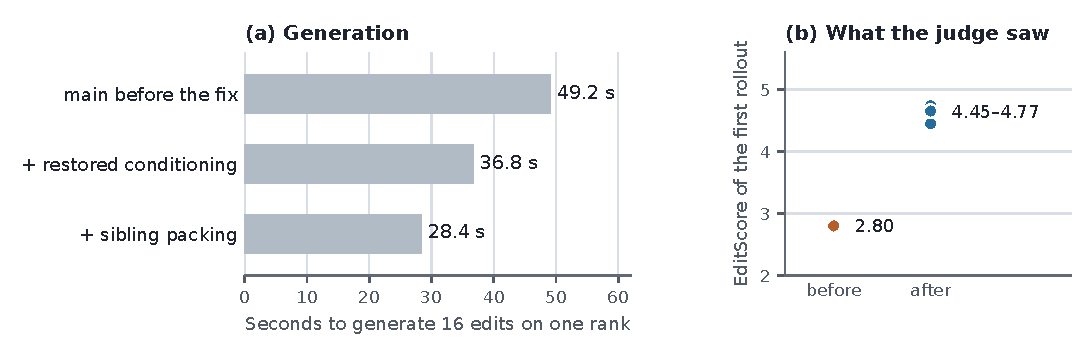
\includegraphics[width=\textwidth]{artifacts/reported_results/2026-10-04-rollout-fidelity/figures/rollout_chain.pdf}
\caption{The image-editing rollout before and after the changes, on one eight-GPU node with a remote EditScore judge. Left: seconds to generate one rank's sixteen edits. Right: the mean judge score of the first rollout, which no optimizer step has yet influenced; the points after the fix are separate runs of the same first batch.}
\label{fig:fidelity-chain}
\end{figure}

\begin{table}[H]
\caption{Image editing with LoRA on one eight-GPU H20 node, BAGEL through vLLM-Omni, sixteen prompts with eight samples each at $512\times512$, EditScore 8B on a second node. Generation is the slowest rank's seconds for its sixteen rows. The reward column is the mean judge score of the first rollout on the same prompts, before any optimizer step.}
\label{tab:fidelity-chain}
\centering
\small
% Generated by artifacts/reported_results/2026-10-04-rollout-fidelity/generate.py; do not edit.
\begin{tabularx}{\textwidth}{@{}Xrrrr@{}}
\toprule
Rollout path & Rollouts & Generation (s) & vs.\ \texttt{main} & First-rollout reward \\
\midrule
\texttt{main} before the fix & 1 & 49.2 & -- & 2.80 \\
+ restored it2i conditioning (\#547) & 1 & 36.8 & $-$25\% & 4.62 \\
+ per-group canvas (\#549) & 1 & 36.5 & $-$26\% & 4.77 \\
+ sibling packing (\#550) & 4 & 28.4 & $-$42\% & 4.45--4.74 \\
\bottomrule
\end{tabularx}

\end{table}

Table~\ref{tab:fidelity-chain} puts the four changes on one workload: generation per rank falls \RFTotalSaving{}, from \RFMainGenerate{}\,s to \RFPackGenerate{}\,s, and the first rollout's judge score settles between \RFPostFixRewardMin{} and \RFPostFixRewardMax{} instead of \RFMainReward{}.
The first-update ratio stays within $10^{-4}$ of 1 throughout, and the layout check passes on every replay of every arm, including the ones where a micro-batch cuts a group.
These are one to four rollouts per arm on a single workload shape: they establish the direction and size of each change on this path, not a distribution.

The consequence for Section~\ref{sec:reward} should be stated plainly.
Its image-editing measurements were taken on this path before the conditioning was restored, so their generation phase carries the engine's own, more expensive prefix.
The reward cost in those tables is unaffected---the judge scored the same number of images---so a corrected baseline would spend relatively more of its rollout on reward than Section~\ref{sec:reward} reports, and the overlap it measures would matter more rather than less.
We have not re-run that study on the corrected path.

\subsection{The long tail that mixed resolution exposes}
\label{sec:fidelity-tail}

Once a rollout can mix canvases, the assignment of rows to ranks stops being neutral.
Today it is the data-parallel split: prompts in order, equal row counts, no attention to cost.
On a dataset whose canvases are drawn from a production-like distribution---half small, a fifth at the default, a four-fold span in tokens---the steady text-to-image rollout spent \RFTtoiIdle{} of its rollout window with at least one rank idle, waiting on a rank that had drawn the expensive prompts.

We measured what a cost-aware assignment recovers.
A coordinator hands each rank units of work from a queue ordered by an estimated cost, and an idle rank may take the cheapest unit from the busiest rank's queue; rows are restored to their original order by identifier before credit assignment, so the trajectory the trainer sees is unchanged.
Table~\ref{tab:fidelity-tail} reports the steady rollout of each arm.

\begin{table}[H]
\caption{Assignment of mixed-canvas work to ranks, second rollout of each arm, on one eight-GPU node. ``Idle'' is the fraction of the rollout window in which at least one rank has finished and waits. The cost estimate is image tokens. This mechanism is on a branch with no pull request.}
\label{tab:fidelity-tail}
\centering
\small
% Generated by artifacts/reported_results/2026-10-04-rollout-fidelity/generate.py; do not edit.
\begin{tabularx}{\textwidth}{@{}Xrrrr@{}}
\toprule
Assignment & Rollout + reward (s) & Slowest rank (s) & Mean rank (s) & Idle \\
\midrule
\multicolumn{5}{@{}l}{t2i, in-process PickScore} \\
Prompt-order shards (today) & 150.2 & 147.2 & 103.8 & 29\% \\
Cost-balanced shards & 108.6 & 105.8 & 103.7 & 2\% \\
Cost-balanced shards with stealing & 108.7 & 105.8 & 103.6 & 2\% \\
\midrule
\multicolumn{5}{@{}l}{it2i, EditScore 8B on another node} \\
Prompt-order shards (today) & 99.3 & 91.0 & 63.7 & 29\% \\
Prompt-order shards, reward overlapped & 93.7 & 91.2 & 63.7 & 30\% \\
Cost-balanced shards with stealing & 77.4 & 68.0 & 63.7 & 6\% \\
Cost-balanced with stealing, reward overlapped & 71.5 & 68.1 & 63.8 & 5\% \\
\midrule
\multicolumn{5}{@{}l}{it2i, EditScore 72B on another node} \\
Prompt-order shards (today) & 128.4 & 90.8 & 63.7 & 21\% \\
Cost-balanced with stealing, reward overlapped & 131.1 & 68.4 & 63.8 & 8\% \\
\bottomrule
\end{tabularx}

\end{table}

Three readings, each from two rollouts of each arm.
Balancing recovers most of the tail where the cost estimate is good: text-to-image falls from \RFTtoiBase{}\,s to \RFTtoiBalanced{}\,s and idle time from \RFTtoiIdle{} to 2\%, while the mean per-rank generation time is unchanged at about 104\,s, so the work was redistributed rather than reduced.
Stealing is insurance against a wrong estimate rather than a gain in its own right: with a good cost model it never triggered, and with a deliberately naive one that counts rows and ignores the canvas, which gave back \RFNaiveGap{}\,s of the balancing gain, it recovered \RFStealRecovered{} of them (\RFNaiveBalanced{}\,s to \RFNaiveSteal{}\,s).
And the two mechanisms compose with the reward schedule of Section~\ref{sec:reward}: against a judge with headroom, overlapping reward alone took the editing rollout from \RFSmallBase{}\,s to \RFSmallOverlap{}\,s, the cost-aware assignment alone to \RFSmallSteal{}\,s, and both together to \RFSmallBoth{}\,s, or \RFSmallBothSaving{}.

The negative result is the useful one.
Against the saturated 72B judge, balancing made the step \emph{slower}: \RFLargeBase{}\,s against \RFLargeSteal{}\,s in the steady rollout and \RFLargeFirstBase{}\,s against \RFLargeFirstSteal{}\,s in the first.
It still flattened generation---the slowest rank fell from \RFLargeTail{}\,s to \RFLargeTailSteal{}\,s---but that is exactly the harm: with ranks finishing together they reach the judge together, and the queueing that the uneven baseline had spread out now happens all at once.
This is the same mechanism that Section~\ref{sec:reward-results} found behind micro-batching's gain, read in reverse, and it says that such a scheduler must be gated on whether the reward has headroom rather than enabled by default.
A second cost, measured and not yet addressed: the training phase ran 3--9\% slower, because after the rows are restored to their original order a rank replays rows that another rank generated and their latents cross workers.
The step is still shorter overall where the scheduler helps, but an assignment that also followed the rows into training would not pay this.
None of this is proposed yet.
